\documentclass[11pt]{article}
\usepackage[left=1in,right=1in,top=1in,bottom=1in]{geometry}
\usepackage{amsmath}
\let\verbatiminput=\verbatimtabinput
\def\verbatimtabsize{4\relax}
\usepackage{array}
\usepackage{booktabs}
\usepackage{minted}
\usepackage{parskip}
\usepackage{float}

\usepackage{color}
\definecolor{rltred}{rgb}{0.75,0,0}
\definecolor{rltgreen}{rgb}{0,0.5,0}
\definecolor{rltblue}{rgb}{0,0,0.75}

\usepackage[%pdftex,
    colorlinks=true,
    urlcolor=rltblue,               % \href{...}{...}
    anchorcolor=rltbrightblue,
    filecolor=rltgreen,             % \href*{...}
    linkcolor=rltred,               % \ref{...} and \pageref{...}
    menucolor=webdarkblue,
    citecolor=webbrightgreen,
    pagebackref,
    pdfpagemode=UseNone,
    bookmarksopen=true]{hyperref}
\usepackage{graphicx, subcaption}

\begin{document}
\begin{center}
  \textbf{\LARGE EE 240C Project: ADC Modeling and Non-Ideality Analysis}
\end{center}

\section{Choice of Architecture}
The desired specs for the ADC are listed in Table \ref{tab:adc_specs}.

\begin{table}[hbt]
  \begin{center}
    \caption{ADC Specifications}
    \label{tab:adc_specs}
    \begin{tabular}{l l}
      \toprule
      \textbf{Parameter} & \textbf{Value} \\
      \midrule
      Bandwidth & $\geq 12.5$ MHz\\
      Dynamic Range & $\geq 70$ dB\\
      Signal to Noise and Distortion Ratio & $\geq 65$ dB\\
      Power Consumption & minimize \\
      \bottomrule
    \end{tabular}
  \end{center}
\end{table}

I looked at Boris Murmann's 2012 ADC survey. His plots are in Figure \ref{fig:adc_survey}.

\begin{figure}[h]
  \centering
  \begin{subfigure}[t]{0.48\textwidth}
    \centering
    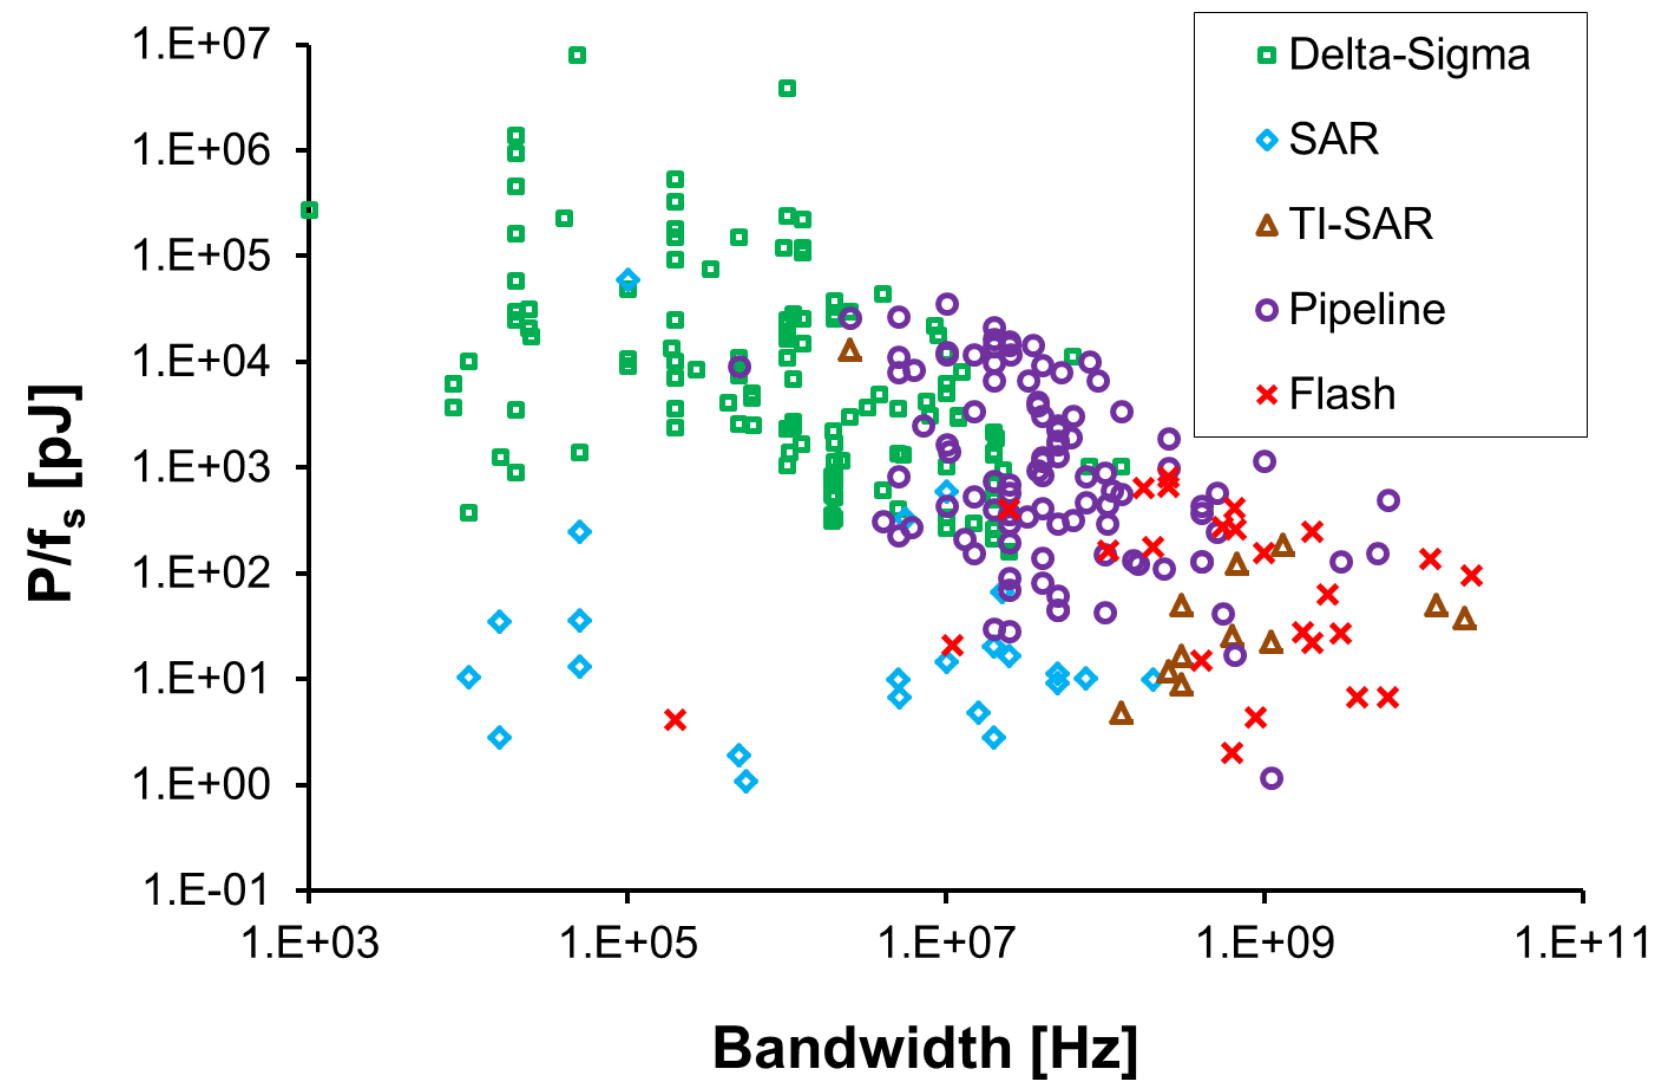
\includegraphics[height=2in]{figs/bw_vs_energy.png}
  \end{subfigure}
  \hfill
  \begin{subfigure}[t]{0.48\textwidth}
    \centering
    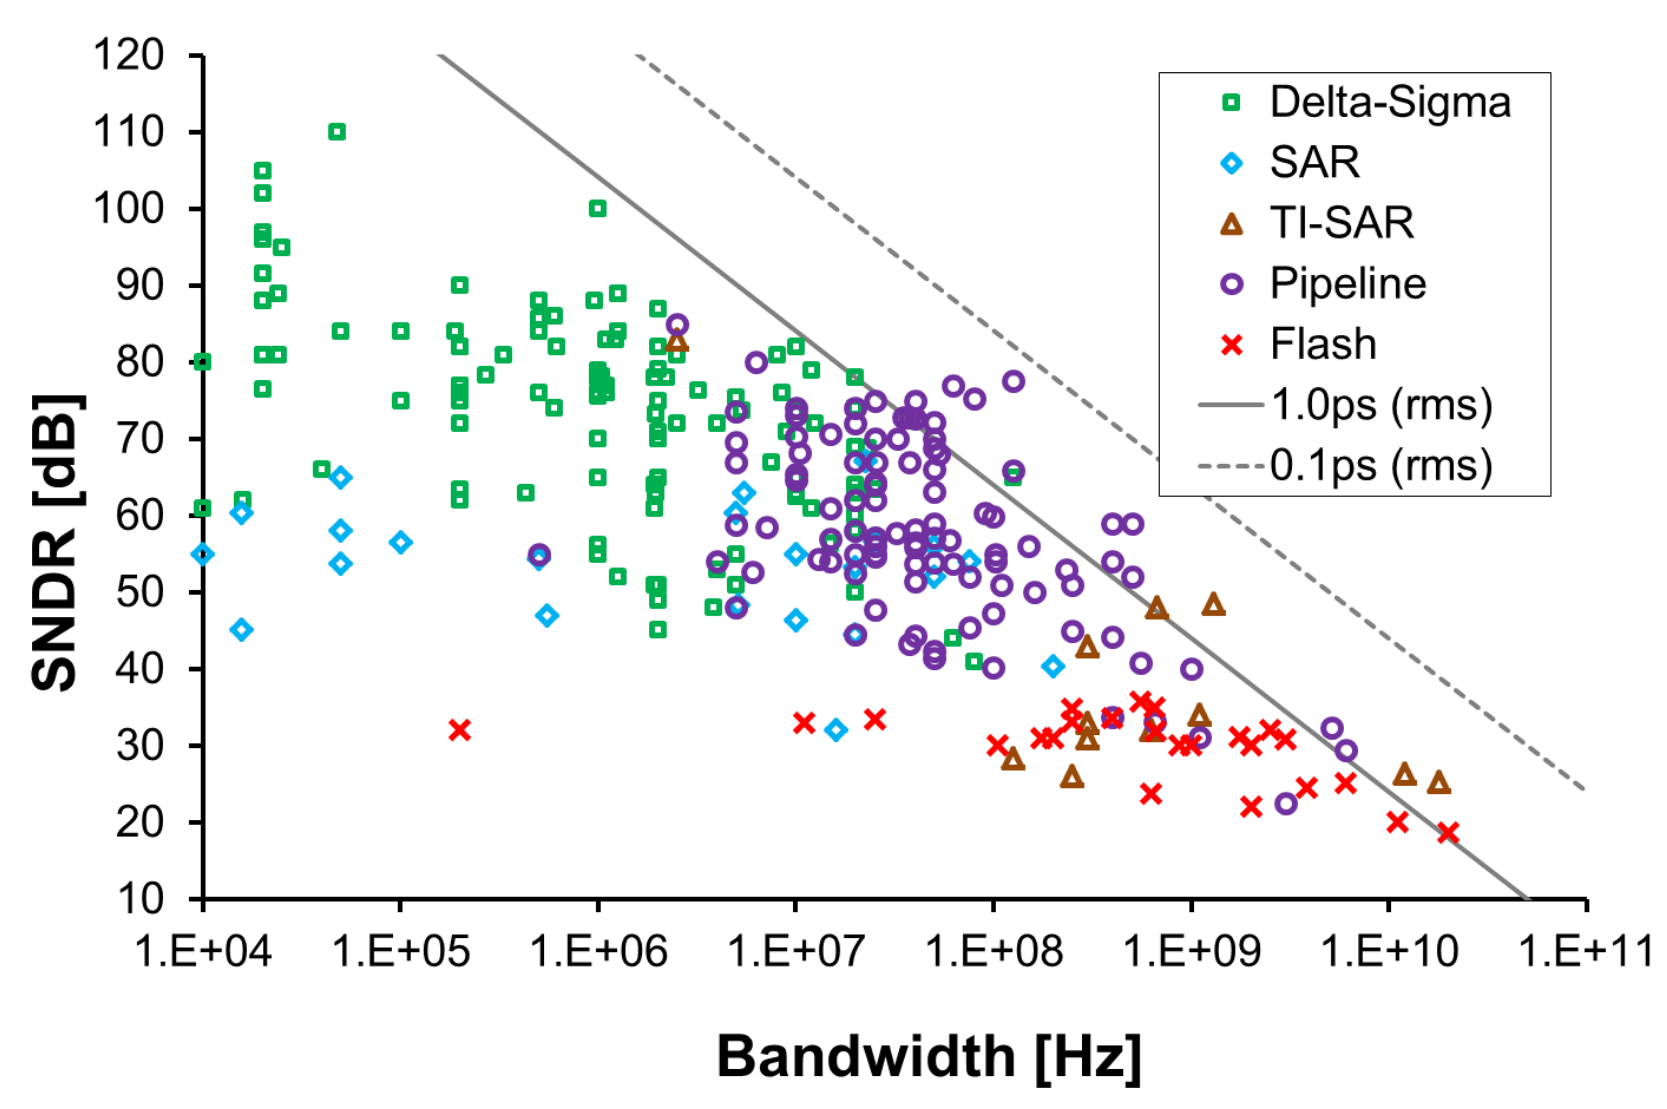
\includegraphics[height=2in]{figs/bw_vs_sndr.png}
  \end{subfigure}
  \caption{Plots from Murmann's (2012) ADC survey}
  \label{fig:adc_survey}
\end{figure}

Clearly a flash architecture cannot reasonably meet the SNDR requirement and would be more suitable for a higher bandwidth requirement.
The SAR architecture seems to deliver the best power efficiency, but it looks like the SOTA SAR ADCs cannot achieve a SNDR higher than 70 dB which makes achieving 65 dB a difficult proposition for this architecture.

The dynamic range spec translates to a 12-bit ADC, and scanning the table of ADC papers from Murmann's spreadsheet, either a pipeline or sigma-delta architecture seems appropriate.
% slide 32 lecture 9
According to figures from Pavan ("Understanding Delta-Sigma ADCs"), the sigma-delta ADC requires an oversampling ratio of 32-64 for a low-order modulator (2-3) and an OSR of 16-32 for a high-order modulator (4-6) to achieve SQNR above 65 dB.
This figure doesn't account for other noise sources from the SC stages used for error feedback, the sampling capacitor, or distortion.
This means the ADC has to run at $f_{adc} = 12.5 \cdot 2 \cdot \text{OSR}$ which is 400 - 800 MHz, imposing additional power requirements on the SAH stage to achieve settling time requirements.

In contrast the SAH and gain stages of the pipeline ADC can run at the Nyquist rate, and it should be able to achieve the SNDR spec.
I will design a model of a pipeline ADC.

\section{Pipeline ADC Modeling}


\end{document}
